\section{Experiments}
\begin{frame}{Static \& Dynamic Experiments}
  \begin{itemize}
    \item Diversity measures
      \begin{itemize}
        \item NNTD ($100 \cdot 100 \cdot t$ for snake)
        \item Levenschtein distance ($450^2 \cdot 100^2 = 2$ billion for snake)
        \item Hamming distance ($450 \cdot 100^2 = 4.5$ million for snake) % normalized average between all pairs of individuals
      \end{itemize}
    \item Evaluation environments
      \begin{itemize}
        \item Static
        \item Dynamic
      \end{itemize}
    \item Why did we choose this setup
    \item What are they good for?
  \end{itemize}
\end{frame}

\begin{frame}{Static Results}
  
\end{frame}

\begin{frame}{Dynamic Results}
  
\end{frame}

\section{Conclusion}
\begin{frame}{Conclusion}
  \begin{itemize}
    \item What can we say from our experiments?
      % NNTD outperforms a genetic and a fitness-based measure
      % The phenotypic fitness-based measure of ave unreliable
      % Genotypic 
    \item Many, many factors and variables influence results
  \end{itemize}
\end{frame}

\section{Future Work}
\begin{frame}{Future Work}
  \begin{itemize}
    \item Comparison to other diversity measures
    \item Determining random inputs % their range and size
    \item Understanding the difference between Hamming distance and NNTD
    \item Different bucket classification algorithms
  \end{itemize}
\end{frame}

\begin{frame}{Bucket classification}
  \begin{columns}
    \column{0.5\paperwidth}
    \begin{itemize}
      \item NNTD classifies output neurons based on boolean output
      \item It's possible to classify by a singular output's range instead
      \item Such a method would expand range of problems
    \end{itemize}

    \column{0.5\paperwidth}
    \begin{figure}[htbp]
      \centering
      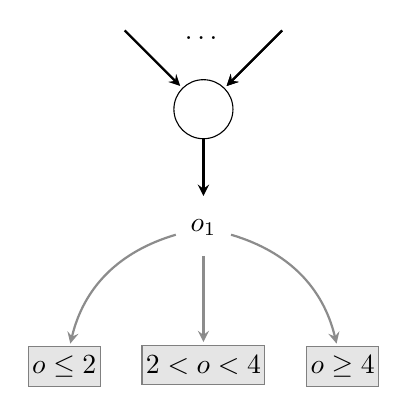
\begin{tikzpicture}
  [->, >=stealth, shorten >=1pt,auto,node distance=2cm,
    align=center,
    neuron/.style={%
      circle, draw, minimum size=0.75cm
    },
    invis/.style={%
      circle
    },
    bucket/.style={%
      rectangle,draw=black!50,fill=black!10,
      minimum size=5mm,inner sep=0.5mm
    },
  ]

  \node[neuron] (o) {};
  \node[invis] (o2) [below of=o, node distance=1.5cm] {$o_1$};

  \draw[->,thick] (o) -- (o2);

  \node[bucket] (b2) [below of=o2, node distance=1.75cm] {$2 < o < 4$};
  \node[bucket] (b1) [below left of=o2, node distance=2.5cm] {$o\leq2$};
  \node[bucket] (b3) [below right of=o2, node distance=2.5cm] {$o\geq4$};

  \draw[->,thick] ++(-1,1) -- (o); 
  \draw[->,thick] ++(1,1) -- (o); 
  \draw[->,thick] ++(1,1) -- (o) node[above=0.75cm] {\dots};

  \path[->,thick,gray,opacity=0.9]
  (o2) edge [bend right] (b1)
       edge (b2)
       edge [bend left] (b3);

\end{tikzpicture}

    \end{figure}
  \end{columns}
\end{frame}
